% !TEX root = main.tex

\section{Experiments}
\label{sec:experiments}
In this section, we conduct experiments to evaluate the performance of I$^2$GL. Note that AIGL can be applied for not only Ethereum, but also other cryptocurrencies that support smart contracts.

\subsection{Data Collection}
We collect data by running a  Ethereum client\footnote{Parity Ethereum Client, https://www.parity.io/ethereum/}, which synchronize all historical transaction records from the Ethereum blockchain. We choose the transaction records during January 1, 2018 and March 31, 2018, including 116,293,867 external transactions and internal transactions in total, as the input of graph construction. This is the most active period with various activities. By parsing these transactions, we obtain 16,599,825 active accounts, including 14,450,993 EOAs and 2,148,831 SCs\footnote{Besides the EOAs and CAs, we abstract a system account which is in charge of paying out ETH bonuses to miners.}.

Specially, \textcolor{red}{\{unclear\}we extend the pre-processing scheme to adapt our model} by constructing four relation graphs, which contains ETH transfer graph, contract creation graph, contract invocation graph and mining reward graph. In each graph, repeated edges between the same node pair are merged using the method introduced in Section \ref{sec:approach}.

%Last, a set of accounts with label introduced before is provided to train the model and evaluate classification accuracy. It is hard to reveal the identity of addresses since the anonymity of blockchain. We obtain these labeled examples in two ways, \emph{Etherscan}\footnote{Etherscan LabelCloud, https://etherscan.io/labelcloud} and \emph{Searchain}\footnote{Searchain, http://www.searchain.io/}. In the label set, the number of samples of each category is 100.

\subsection{Identity Categorization}
Since I$^2$GL uses a semi-supervised learning method, a small set of labeled accounts should be prepared for training. We obtain these labeled examples from \emph{Etherscan}\footnote{Etherscan LabelCloud, https://etherscan.io/labelcloud} and \emph{Searchain}\footnote{Searchain, http://www.searchain.io/}. TABLE~\ref{table:identity} shows the taxonomy of Ethereum accounts used in our experiments. Even though new account types emerge as the development of Ethereum, I$^2$GL can be easily extended to handle them. The details of some major account types are depicted as follows.
 %It is hard to reveal the identity of addresses since the anonymity of blockchain.  %In the label set, the number of samples of each category is 100.

\noindent 1) \emph{Miner \& Mining Pool}
The existing implementation of Ethereum blockchain use the \emph{Proof-of-Work (PoW)} protocol, similar with Bitcoin. The \emph{miners} are the individuals or groups who validate transaction information by solving the cryptographic puzzles. Whoever is the first to find a valid hash of block will get the reward in the form of ETH which is paid by users sending transactions. To improve mining efficiency, miners work together to solve the PoW problems by registering at a special institution named \emph{mining pool}, which aggregates all the registrants' computing power to solve mining problems and distributes the reward to registrants according to their proportion of contributed computing power. Up to March 2018, top $3$ mining pools occupy more than 65\% of hash rate in Ethereum\footnote{Investoon, https://investoon.com/charts/mining/eth.}.

\noindent 2) \emph{Exchange}
The exchanges are the platforms for trading ETH and other cryptocurrencies, and they play important roles in the Ethereum ecosystem. Most of cryptocurrency trading is done through centralized exchanges such as Binance, Huobi, OKEX, etc\footnote{``Top 100 Cryptocurrency Exchanges by Trade Volume'', https://coinmarketcap.com/rankings/exchanges}. The centralized exchange allocates a deposit address to each user who wants to make transactions via the exchange. These addresses are called \emph{exchange deposits} and belong to the exchange since users do not have the private key of these addresses. In the recharge process, users transfer coins to the given deposit addresses from their own wallets and these coins will be transferred to the \emph{exchange root} address automatically. In turn, users send requests to exchange to withdraw their coins from an address called \emph{exchange withdrawal}. And in most cases, the exchange root and exchange withdrawal mean the same address.

%The exchanges can be categorized into centralized exchanges and decentralized exchanges (also known as DEXs) according to their architectures.

%The exchange charges the user a commission for both recharge and withdraw services.

%The DEXs are a new technology that facilitate cryptocurrency trading on a distributed ledger. Being completely on-chain, all orders interact with each other directly through the blockchain. This makes it fully decentralized, but also expensive and slow. Besides, another difference is that user will get a new address with corresponding private key when registers to the DEX, which means the address belongs to user itself instead of exchange.

 %User calls the smart contract in the decentralized exchange address to start a transaction. Intuitively, the transaction will take a long time for making match and confirming compared with in centralized way.

%Since most ERC-20 token transactions happen via smart contracts and in a decentralized mechanism, some big exchanges which support both ETH and ERC-20 token transaction (e.g., Binance and Huobi) are mixture of centralized and decentralized exchange.


\noindent 3) \emph{ERC-20 \& ICO}
As a technical standard on Ethereum, ERC-20 defines a common list of rules that an Ethereum token has to implement, giving developers the ability to program new tokens within the Ethereum ecosystem. Such ERC-20 token transfer happens in specific contract which is called \emph{ERC-20 token contract}. The ERC-20 token standard becames popular with crowdfunding companies working on ICO cases due to the simplicity of deployment, together with its potential for interoperability with other Ethereum token standards~\cite{erc-20}. Up to July 26 2018, there were more than 103,621 ERC-20 token contracts\footnote{Etherscan Token Tracker Page, https://etherscan.io/tokens}. Some successful ERC-20 token sales are EOS, Filecoin, Bancor, Qash, and Nebulas, raising over 60 million each\footnote{``Token Data, data and analytics for all ICO's and tokens", https://www.tokendata.io}. Participants in the initial ICO round are \emph{primary market investors} who buy the ERC-20 token from ERC-20 smart contracts of the crowdfunding companies. And these addresses used for ETH token holding are called \emph{ICO wallets}.

\noindent 4) \emph{Phish/Hack}
Since virtual property transactions are now becoming increasingly common, but lead to many security issues. At the same time, the frauds associated with ETH and ERC-20 tokens have also increased. We call these addresses related to frauds \emph{Phishes/Hacks}. According to Ethersacan, there are more than $2500$ addresses are labeled as Phishes/Hacks, which takes up the highest proportion. Most of them are disguised as ERC-20 token sales or DApps such as casino. 

\begin{table}[t]
\caption{Typical Account Identities}
\begin{center}
\begin{tabular}{c|c|l}
\hline
\textbf{Identity} & \textbf{Type}& \textbf{Description} \\
\hline
Miner & EOA & \tabincell{l}{Node who takes part in the block \\validation process} \\ \hline
Mining Pool & EOA & \tabincell{l}{The pooling of resources by miners, \\who share their processing power \\over a network}\\ \hline
Token Contract & CA & \tabincell{l}{Smart contract that allows customers \\to transfer ERC-20 tokens} \\ \hline
Investor & EOA & \tabincell{l}{Large holder of ETH, who usually \\got in early on ICOs} \\ \hline
ICO Wallet & EOA/CA & \tabincell{l}{ETH holding of token team, typically \\raised from ICOs} \\ \hline
Exchange Deposit & EOA/CA & \tabincell{l}{Address for user to deposit ETH at \\exchange} \\ \hline
Exchange Root & EOA/CA & \tabincell{l}{Address collect ETH from deposit \\addresses and withdraw ETH to users} \\ \hline
Phish/Hack & EOA/CA & \tabincell{l}{Fraud address related to phishing and \\hack} \\ \hline
%\multicolumn{4}{l}{$^{\mathrm{a}}$Sample of a Table footnote.}
\end{tabular}
\label{table:identity}
\end{center}
\end{table}


%Phishing is the name given to the latest online scam where millions of unwary Americans are getting their identities stolen.

%We've seen increased use of sophisticated forms and letterhead to send what appears to be legitimate World Bank Group correspondence, as well as several schemes that reference the Bank.


\subsection{Experiment Setting}
We compare I$^2$GL against state-of-the-art DeepWalk~\cite{perozzi2014deepwalk}, PARW~\cite{wu2012learning} and rGCN~\cite{schlichtkrull2018modeling}. DeepWalk is an embedding technique using random walks on graphs to obtain node representations. Like I$^2$GL, rGCN tackles node representation by defining a convolution operator on graph. PARW is a label propagation method based on partially absorbing random walks. Note that DeepWalk is an unsupervised method, a logistic regression model is added for classification. Unless otherwise noted, all the GCN-based hidden layers have 16 units. Models are trained with Adam optimizer for 100 epochs, and $dropout\_rate=0.5$ is used to avoid overfitting. All embedding and classification programs were run on the server, with an Intel Xeon E5 CPU of 55 processors and 128GB of memory. The GPU used for deep learning is Nvidia 1080.

\begin{table*}
\footnotesize
\centering
\caption{Identity Classification Results}
\resizebox{\textwidth}{25mm}{
\begin{tabular}{l|ccc|ccc|ccc|ccc}
\toprule
 & \multicolumn{3}{c|}{DeepWalk} & \multicolumn{3}{c|}{PARW} & \multicolumn{3}{c|}{rGCN} & \multicolumn{3}{c}{I$^2$GL} \\
\midrule
& \textbf{Precision} & \textbf{Recall} & $\mathbf{F_1}$ & \textbf{Precision} & \textbf{Recall} & $\mathbf{F_1}$ & \textbf{Precision} & \textbf{Recall} & $\mathbf{F_1}$ &  \textbf{Precision} & \textbf{Recall} & $\mathbf{F_1}$ \\
\midrule
 \vspace{1mm}
 Phish/Hack & 0.609 & 0.394 & 0.479 &0.565 & 0.333 & 0.419 & 0.913& 0.212& 0.344& 0.773& 0.758& 0.765\\
 \vspace{1mm}
 Token Contract & 0.857& 0.735 & 0.791 &0.354& 0.718& 0.475& 0.908& 0.602& 0.724& 0.960& 0.970& 0.965\\
  \vspace{1mm}
 Exchange Deposit & 0.586 & 0.531 & 0.557 &0.692& 0.281& 0.400& 0.688& 0.440& 0.537& 0.567& 0.680& 0.618\\
  \vspace{1mm}
 Exchange Root & 0.647 & 0.759 & 0.698 &0.667& 0.759& 0.710& 0.923& 0.686& 0.787& 0.964& 0.771& 0.857\\
  \vspace{1mm}
 Pool & 0.692 & 0.750 & 0.720 &0.789& 0.625& 0.697& 1.000& 0.727& 0.842& 0.800& 0.727& 0.762\\
  \vspace{1mm}
 Miner & 0.400 & 0.694 & 0.508 &0.667& 0.872& 0.756& 0.867& 0.951& 0.907& 0.857& 0.976& 0.909\\
  \vspace{1mm}
Investor & 0.405 & 0.548 & 0.466 & 0.727& 0.516& 0.604& 0.739& 0.548& 0.630& 0.727& 0.516& 0.604\\
 \vspace{1mm}
 ICO Wallet & 0.364 & 0.353 & 0.358 & 0.630& 0.500& 0.558& 0.546& 0.158& 0.245& 0.759& 0.579& 0.657\\
 \midrule
 average & 0.614 & 0.583 & \bf{0.585} & 0.623& 0.577& \bf{0.570}& 0.848& 0.496& \bf{0.593}& 0.829& 0.792& \bf{0.806}\\
\bottomrule
\end{tabular}
}
\label{table:overall_results}
\end{table*}


\subsection{Experiment Results}
For clarity, we have two assumptions about identity inference: 1) each account is supposed to have a single identity instead of multiple identities, and (2) identity of a certain account does not change. These assumptions are reasonable because even though a participant may have multiple identities (e.g., it can be a miner and an investor simultaneously) in practice, it uses different accounts for these activities, respectively. Because we use transaction records during a period of merely three month, cases of identity conversion is negligible.

We use three metrics, precision, recall and $F_1$ score, to evaluate the performance of different approaches. \textcolor{red}{Precision is the fraction of relevant instances among the retrieved instances, while recall is the fraction of relevant instances that have been retrieved over the total amount of relevant instances. A high precision means the classifier is unlikely to consider accounts with other identities as this identity, while a high recall means that most of accounts in this identity will be recognized.} The $F_1$ score is a measurement that combines precision and recall, which is computed as

\begin{equation}
F_1=(\frac{{precision}^{-1}+{recall}^{-1}}{2})^{-1}=2\cdot\frac{precision \cdot recall}{precision + recall}
\end{equation}

In statistical analysis of label classification, the $F_1$ score is an important indicator since it is the harmonic average of the precision and recall. \textcolor{red}{An ideal classifier has both high precision and recall, thus a high $F_1$ score.}

Results are summarized in TABLE~\ref{table:overall_results}. I$^2$GL outperforms other approaches in average $F_1$ score. Comparing with DeepWalk and PARW, our I$^2$GL achieve higher $F_1$ scores in all labels, because these methods only use the local structure of nodes, but our proposed approach use global structural information and statistic information.

Note that rGCN achieves the highest average precision but a low average recall. Especially, rGCN has the lowest recall of category of Phishes/Hacks, which means that many normal accounts are inferred as threatening in rGCN model. Our method improves the overall performance by adding richer information, i.e., the time of transactions, into the model.

%\subsection{Asymmetric Proximity and Time-Density}
\subsection{Visualization}
I$^2$GL is a graph deep learning approach based on graph embedding, and each node in the graph can be represented as a low-dimensional vector. It allows us to visualize the nodes and gain a better understanding of classification. We illustrate the visualization of DeepWalk, rGCN and AIGL in Fig.~\ref{fig:visualization}. Similar to~\cite{wang2016structural}, we use the 128-dimensional embedding for each method, and apply t-SNE~\cite{maaten2008visualizing} to reduce the dimensionality to 2, so that all nodes can be visualized in a 2-dimensional space.

\begin{figure*}
\centering     %%% not \center
\subfigure[DeepWalk]{\label{fig:a}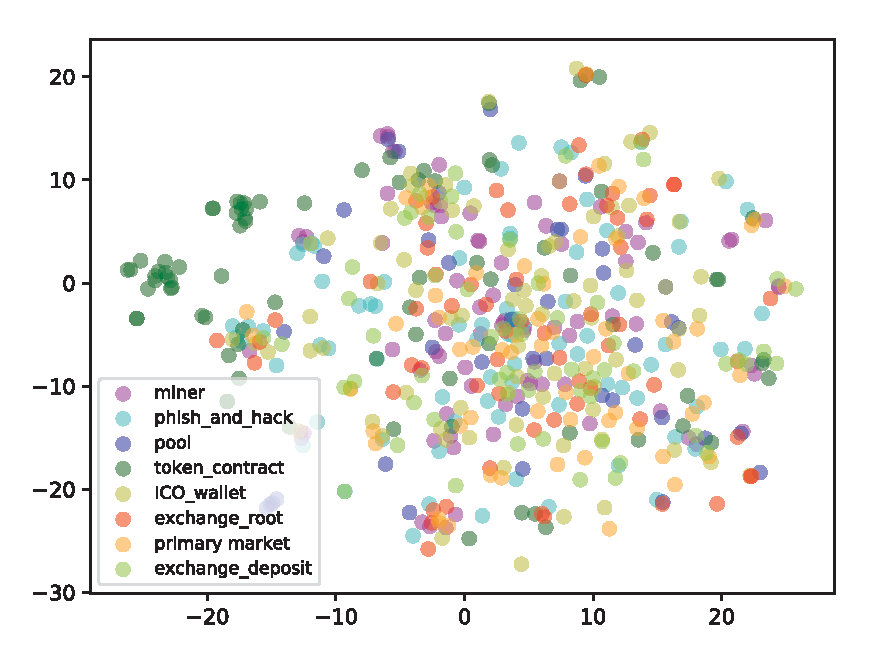
\includegraphics[width=42mm]{fig/rgcn_181_dw_20}}
\subfigure[rGCN]{\label{fig:b}\includegraphics[width=42mm]{fig/rgcn_181_rgcn_20}}
%\subfigure[rGCN+asymmetric proximity]{\label{fig:a}\includegraphics[width=42mm]{fig/rgcn_181_rgcn_181_asym_only_20}}
\subfigure[I$^2$GL]{\label{fig:a}\includegraphics[width=42mm]{fig/rgcn_181_rgcn_ours_20}}
\caption{Visualization of nodes with different labels in 2-dimensional space.}
\label{fig:visualization}
\end{figure*}

We use different colors to denote accounts labelled as different identities. Therefore, in a good embedding result, points with the same color should be grouped together. It can be observed that all GCN based approaches outperform DeepWalk since GCN model well preserves global structure information~\cite{goyal2018graph}. Furthermore, we find that many Phishes/Hacks accounts are usually disguised as ICO wallets and exchange deposits because their points overlap in Fig \ref{fig:visualization}(c).

\subsection{Deeper Analysis}
To investigate the characters of transaction graph, we make further experiments.

\begin{figure*}
\setlength{\tabcolsep}{-5pt}
  \centering
  \begin{tabular}{cccc}
	\subfigure[Multi-Adjacencies]{
		\label{fig:multi_relation_result}
  \begin{tikzpicture}
\begin{axis}[avg]
\addplot+ [black, fill=blue!30, error bars/.cd,y dir=both,y explicit] table [
col sep=comma,
  x=x,
  y=a,
  y error plus expr=\thisrow{a-max}-\thisrow{a},
  y error minus expr=\thisrow{a}-\thisrow{a-min},
]{\multirelationtable};

\addplot+ [black, fill=white, postaction={pattern=north east lines}, error bars/.cd,y dir=both,y explicit] table [
col sep=comma,
  x=x,
  y=b,
  y error plus expr=\thisrow{b-max}-\thisrow{b},
  y error minus expr=\thisrow{b}-\thisrow{b-min},
]{\multirelationtable};

\legend{I$^2$GL$_{\text{sR}}$, I$^2$GL$_{\text{mR}}$};

\end{axis}
\end{tikzpicture}

    } &
	\subfigure[Second-order proximity]{
		\label{fig:second-oder_result}
  \begin{tikzpicture}
\begin{axis}[avg]
\addplot+ [black, fill=blue!30, error bars/.cd,y dir=both,y explicit] table [
col sep=comma,
  x=x,
  y=a,
  y error plus expr=\thisrow{a-max}-\thisrow{a},
  y error minus expr=\thisrow{a}-\thisrow{a-min},
]{\multilayertable};

\addplot+ [black, fill=white, postaction={pattern=north east lines}, error bars/.cd,y dir=both,y explicit] table [
col sep=comma,
  x=x,
  y=b,
  y error plus expr=\thisrow{b-max}-\thisrow{b},
  y error minus expr=\thisrow{b}-\thisrow{b-min},
]{\multilayertable};

  \legend{\footnotesize{I$^2$GL$_{\text{1L}}$}, I$^2$GL};

\end{axis}
\end{tikzpicture}

    } &
	\subfigure[Asymmetric proximity]{
		\label{fig:asymmetric_order_result}
  \begin{tikzpicture}
\begin{axis}[avg]
\addplot+ [black, fill=blue!30, error bars/.cd,y dir=both,y explicit] table [
col sep=comma,
  x=x,
  y=a,
  y error plus expr=\thisrow{a-max}-\thisrow{a},
  y error minus expr=\thisrow{a}-\thisrow{a-min},
]{\symtable};

\addplot+ [black, fill=white, postaction={pattern=north east lines}, error bars/.cd,y dir=both,y explicit] table [
col sep=comma,
  x=x,
  y=b,
  y error plus expr=\thisrow{b-max}-\thisrow{b},
  y error minus expr=\thisrow{b}-\thisrow{b-min},
]{\symtable};

\legend{I$^2$GL$_{\text{nT,nA}}$, I$^2$GL$_{\text{nT}}$};

\end{axis}
\end{tikzpicture}

    } &
	\subfigure[Time-density]{
		\label{fig:time-density_result}
  \begin{tikzpicture}
\begin{axis}[avg]
\addplot+ [black, fill=blue!30, error bars/.cd,y dir=both,y explicit] table [
col sep=comma,
  x=x,
  y=a,
  y error plus expr=\thisrow{a-max}-\thisrow{a},
  y error minus expr=\thisrow{a}-\thisrow{a-min},
]{\timedensitytable};

\addplot+ [black, fill=white, postaction={pattern=north east lines}, error bars/.cd,y dir=both,y explicit] table [
col sep=comma,
  x=x,
  y=b,
  y error plus expr=\thisrow{b-max}-\thisrow{b},
  y error minus expr=\thisrow{b}-\thisrow{b-min},
]{\timedensitytable};

\legend{I$^2$GL$_{\text{nT}}$, I$^2$GL};

\end{axis}
\end{tikzpicture}

    } \\
  \end{tabular}
\caption{Classification results of diminished I$^2$GLs.}
\label{fig:deeper_analysis}
\end{figure*}

First, we compare the performance of I$^2$GL with single adjacency matrix and single relation (I$^2$GL$_{sR}$ for short) and I$^2$GL with multi-adjacency matrices (I$^2$GL$_{mR}$ for short). Note that both I$^2$GL$_{sR}$ and I$^2$GL$_{mR}$ do not make other enhancements like time-density matrices. As shown in Fig.~\ref{fig:multi_relation_result}, the classification accuracy of I$^2$GL$_{mR}$ increases greatly by introducing multi-adjacency matrices, which indicates that such heterogeneous activities is important in preserving features of transaction graph.

Second, we evaluate the I$^2$GL with 1 layer convolutional network (I$^2$GL$_{1L}$ for short) and I$^2$GL with 2 layers convolutional network, which is complete I$^2$GL. As shown in Fig.~\ref{fig:second-oder_result}, the $F_{1}$ increases $13$\% by preserving second-order proximity, which demonstrates the importance of second-order proximity in the structure of transaction graph. 

Then, we investigate the asymmetric proximity in Ethereum transaction graph, by comparing the I$^2$GL without asymmetric coefficient and time-density matrices (I$^2$GL$_{nT,nA}$ for short) and one without time-density matrices (I$^2$GL$_{nT}$ for short). As shown in Fig.~\ref{fig:asymmetric_order_result}, I$^2$GL$_{nT,nA}$ has higher precision but I$^2$GL$_{nT}$ outperforms in recall and aggregative $F_1$.

Last, we test the performance of I$^2$GL without time-density matrices (I$^2$GL$_{nT}$ for short). As shown in Fig.~\ref{fig:time-density_result}, I$^2$GL outperforms I$^2$GL$_{nT}$ in all indicators. The reason is that different types of accounts have diverse active time distribution, time-density helps to distinguish between them. Also, intensive transactions reflect more typical characteristics, therefore deserve higher weights.
%Preserving asymmetric proximity by adjusting the adjacency matrix, our method greatly improves the robustness between different labels.  % This is because in vanilla rGCN,



%%% Local Variables:
%%% mode: latex
%%% TeX-master: "analysis"
%%% End:
